% !Mode:: "TeX:UTF-8"
\chapter{常见问题}
\label{chapter-faq}
\begin{enumerate}
\item 本模板如何使用?
\label{faq-howtouse}
\begin{itemize}
	\item 按照第2章的要求,先下载和安装相应的软件,推荐使用\TeX{}Live2012或更新的版本;
	\item 下载cls文件;
	\item 使用tex的编辑器或其他编辑器,编写论文,注意保存为UTF-8编码;
	\item xelatex编译。
\end{itemize}
\item 如何将Mathtype的公式转化为\LaTeX{}公式语言?
\label{faq-mathtype2latex}
\begin{itemize}
	\item 安装Mathtype,启动Mathtype;
	\item 转化设置:在菜单Preferences下,选择Translators选项,在弹出的对话框中,
按照如图\ref{fig-fqa-mathtype1}进行设置\footnote{{\heiti 注意}:file下面的两个选项不要选择,
会在转化时会出来很多信息,这些信息对于公式编译没有关系。所以建议不要选,
如若有兴趣的话,可以选中后实验一下。};
\item 在Mathtype中输入公式;
\item 选中公式,复制到\texttt{.tex}的源文件中,编译即可。
\item[{\heiti 注意:}] 使用MathType输入公式然后转化,这样的输入效率比较低,
而且有些LaTeX提供的公式功能,他也无法实现例如:公式的对齐,编号等等,Mathtype适合初学者使用,
建议学习\LaTeX{}公式输入语言。
\end{itemize}
\begin{figure}
\begin{center}
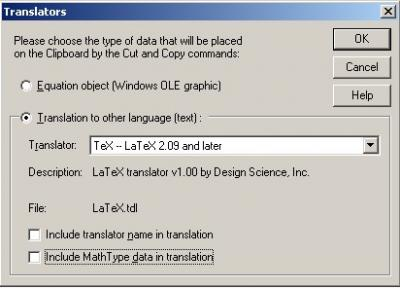
\includegraphics[width=.7\textwidth]{figure/faq-mathtype1.jpg}
\end{center}
\caption{Mathtype中转换设置}\label{fig-fqa-mathtype1}
\end{figure}
\end{enumerate}